\documentclass[landscape]{slides}
\usepackage[landscape, margin=2cm]{geometry}
\usepackage{color}
\usepackage{bm}
\usepackage{graphicx}


\title{Show and Tell: Google Calendar Lifelog}
\author{Adam Johnson - me@adamj.eu}
\date{7th February 2013}

\begin{document}

\maketitle

\begin{slide}

    \textcolor{blue}{\Large{Story}}

    \begin{itemize}
        \item Travelling for 7 months, writing paper diary
    \end{itemize}

    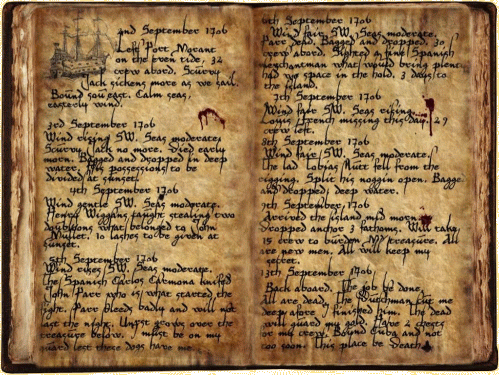
\includegraphics[width=10cm]{capitans-log}

    \begin{itemize}
        \item Loseable! Unsearchable! Sore hand from writing!
    \end{itemize}

\end{slide}


\begin{slide}

    \textcolor{blue}{\Large{Story}}

    \begin{itemize}
        \item Got to San Francisco, bought iPod
    \end{itemize}

    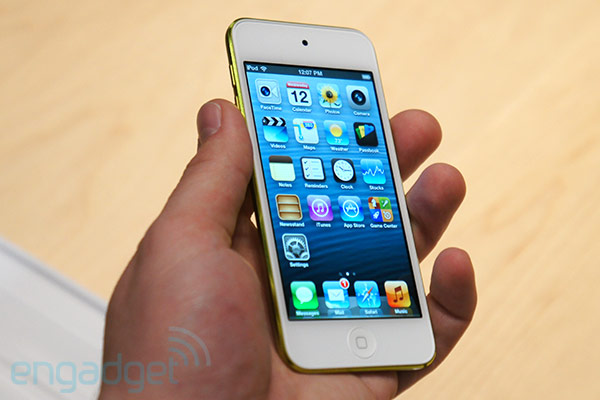
\includegraphics[width=10cm]{new-ipod-touch-2012}

    \begin{itemize}
        \item Backed up, easily searchable, $<1$ minute to write entry
    \end{itemize}

\end{slide}


\begin{slide}

    \textcolor{blue}{\Large{Story}}

    \begin{itemize}
        \item After travelling, continued using Calendar, both as forwards organizational tool and backwards log of what I have done
        \item After a random asthma attack I decided it would make sense to track my inhaler usage: \newline
        \textbf{Jun 22 04:15 - Jun 22 04:15 Inhaler \#drugs}
        \item Steadily more advanced \& varied data
    \end{itemize}

\end{slide}


\begin{slide}

    \textcolor{blue}{\Large{Interfaces}}

    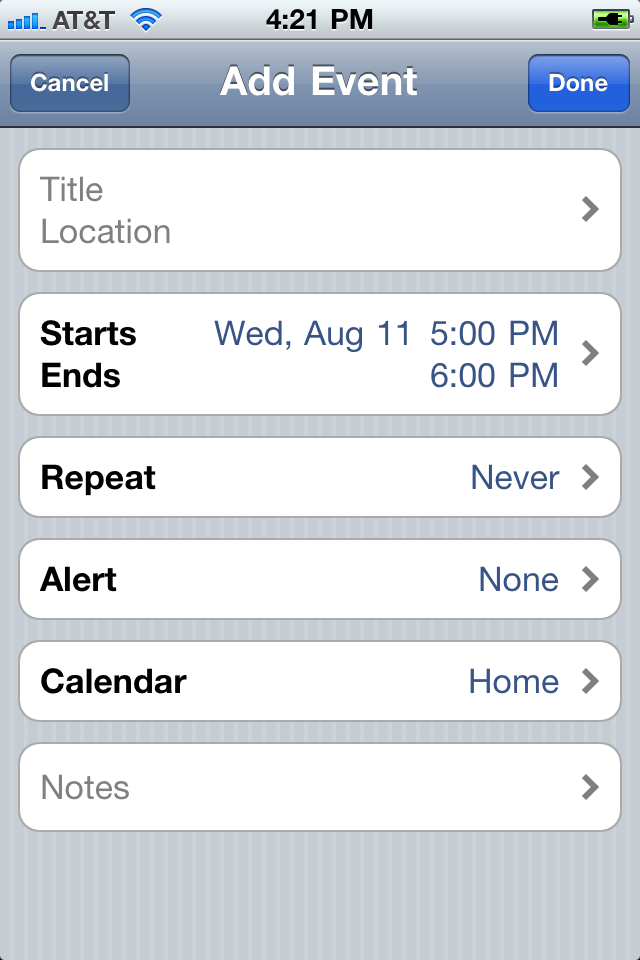
\includegraphics[height=10cm]{ios-calendar-add}

    \begin{itemize}
        \item Too slow!
    \end{itemize}

\end{slide}


\begin{slide}

    \textcolor{blue}{\Large{Interfaces}}

    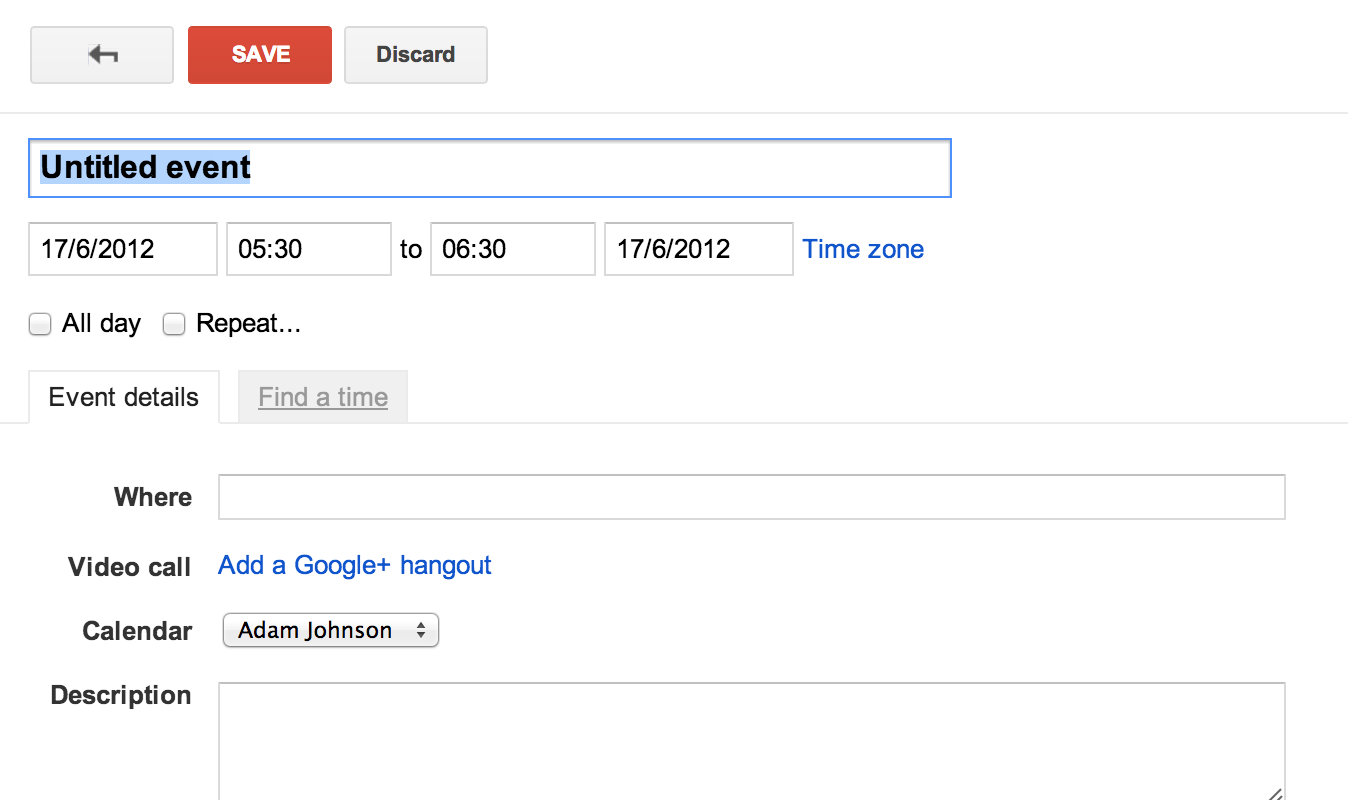
\includegraphics[height=10cm]{google-calendar-add2}

    \begin{itemize}
        \item Too detailed!
    \end{itemize}

\end{slide}


\begin{slide}

    \textcolor{blue}{\Large{Interfaces}}

    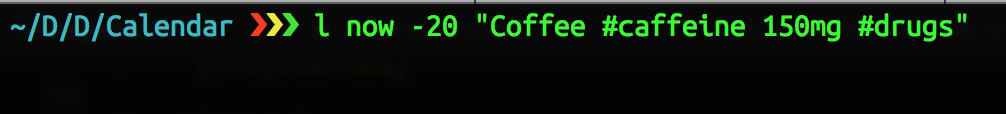
\includegraphics[width=18cm]{cli-calendar-add}

    \begin{itemize}
        \item Just right...

        \item Custom wrapper script to google's commandline interface \newline
        \url{https://github.com/adamchainz/google\_lifelog}

        \item Quick-add syntax + shortcuts to 0-minute events, reverse search repeat
    \end{itemize}

\end{slide}



\begin{slide}

    \textcolor{blue}{\Large{Organization}}

    \begin{itemize}
        \item Hashtags, e.g. \textbf{\#alcohol}, \textbf{\#sleep}, \textbf{\#tv}
        \item Amounts, e.g. \textbf{Double Espresso \#caffeine 150mg \#drugs}
        \item Variables, e.g. \textbf{Rating \#sleepiness=2}
        \item Lazy ``I'll parse it later'' attitude
    \end{itemize}

\end{slide}


\begin{slide}

    \textcolor{blue}{\Large{What I am tracking}}

    \begin{itemize}
        \item Sleep, Drug intake, Hours of work, Social occasions, Exercise, Media consumption, ...
        \item Incredibly easy to start tracking something new
    \end{itemize}


\end{slide}

\begin{slide}
    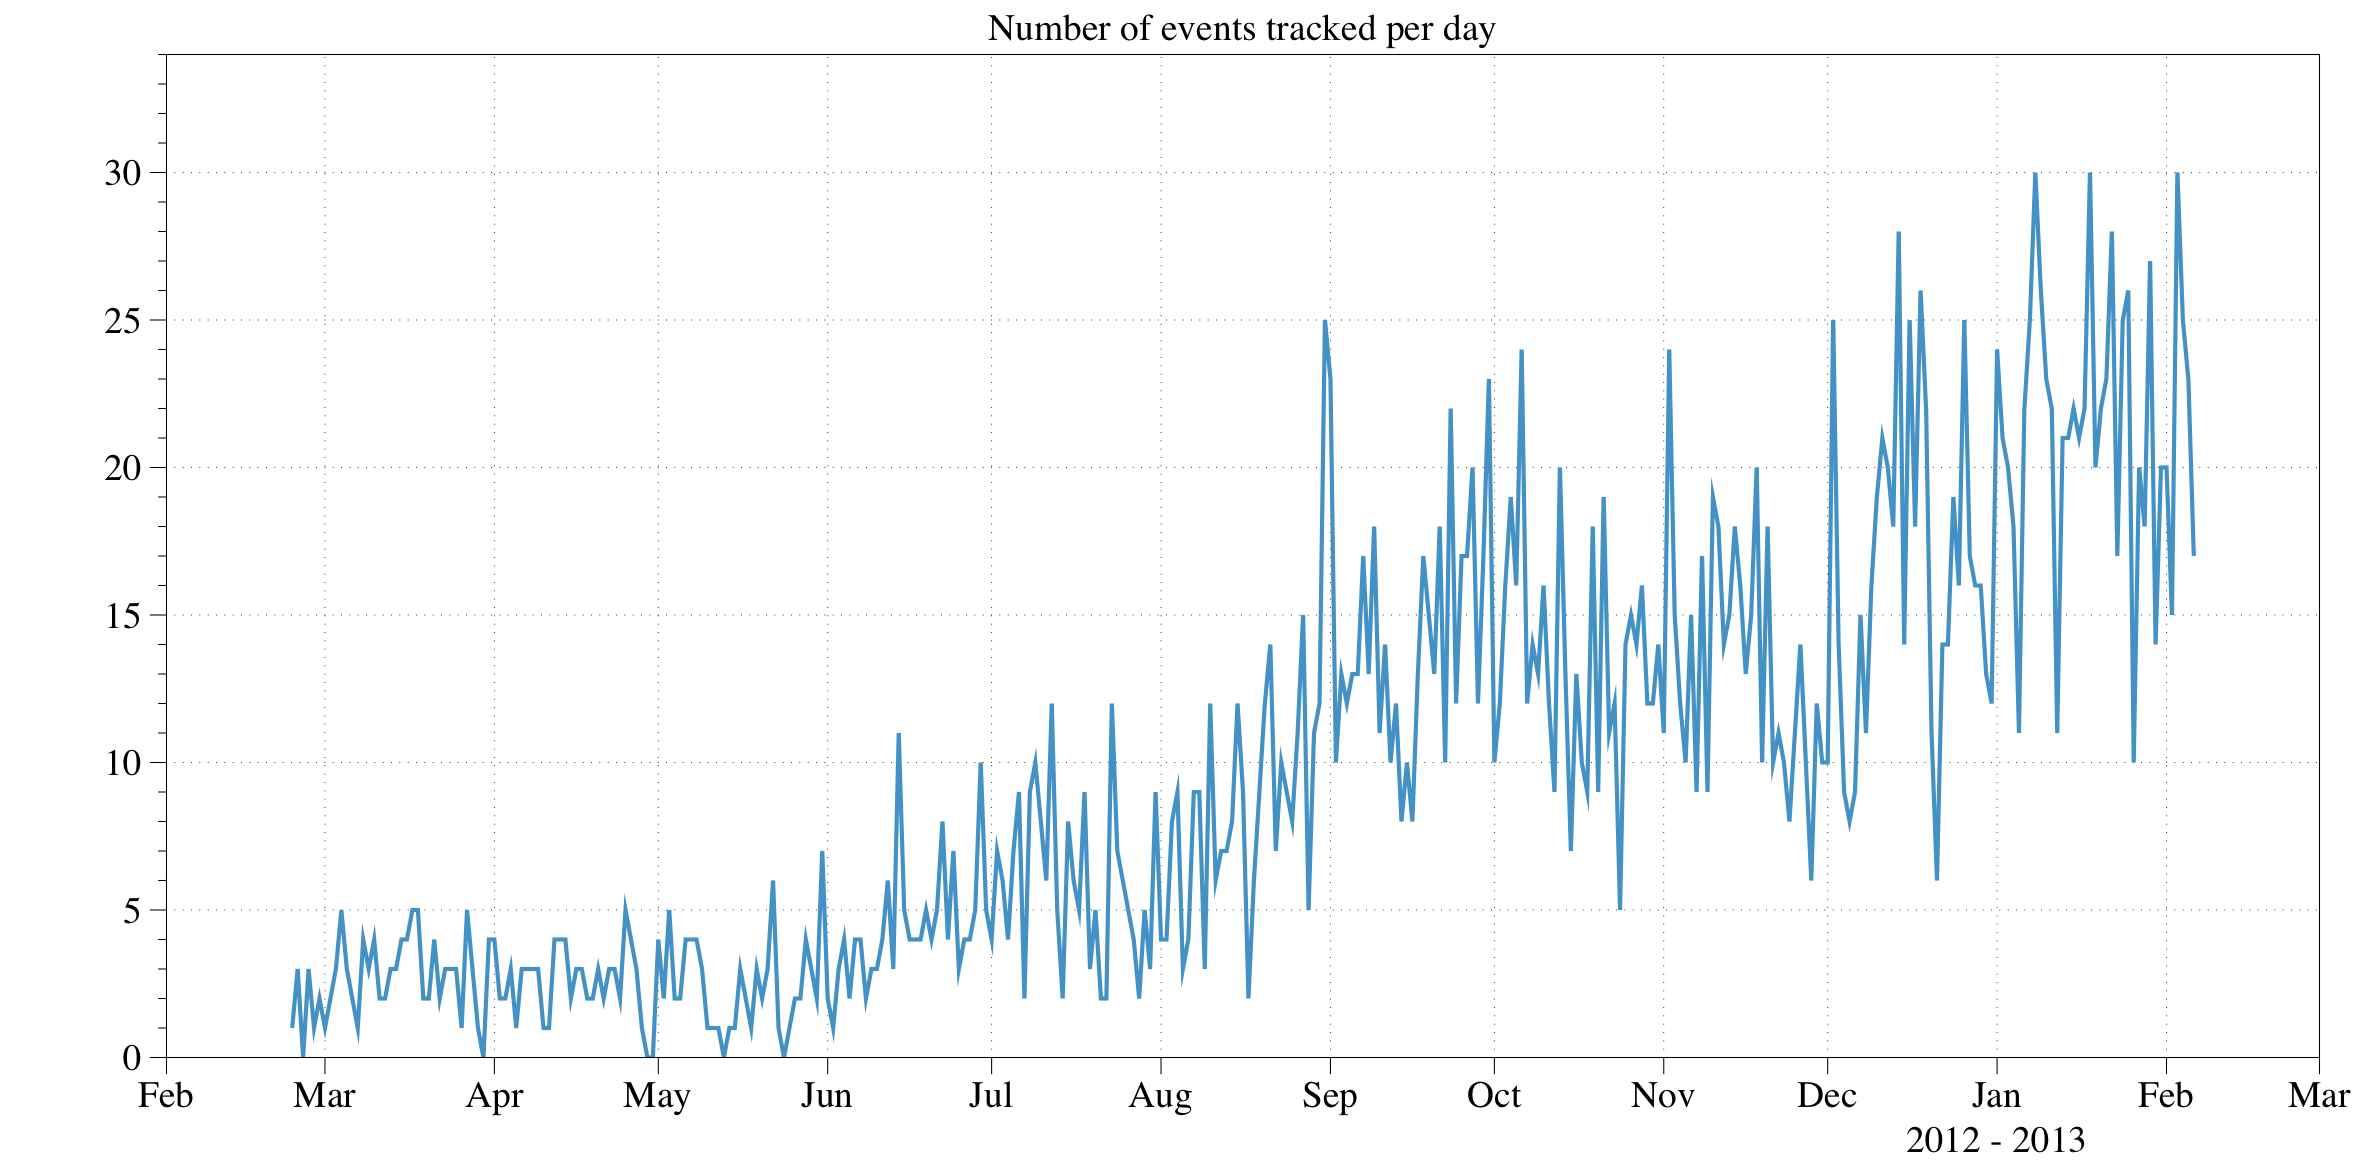
\includegraphics[width=\textwidth]{lifelog-number-per-day}
\end{slide}


\begin{slide}
    \textcolor{blue}{\Large{Analysis}}

    \begin{itemize}
        \item Google let you download the iCal file
        \item Again my little python script provides analysis commands
        \item e.g. \begin{verbatim}lifelog bucket days num ".*"\end{verbatim} was used for previous graph
    \end{itemize}

\end{slide}


\begin{slide}
    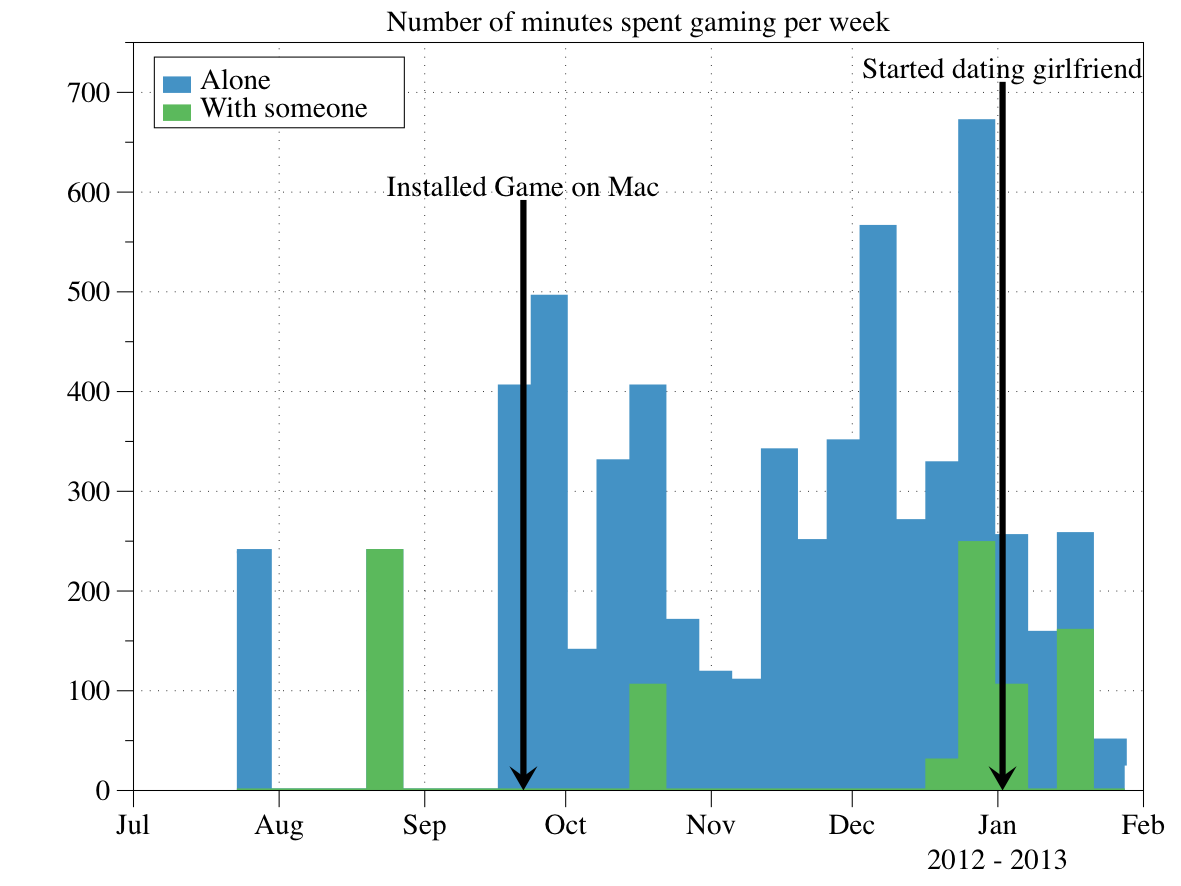
\includegraphics[width=\textwidth]{lifelog-amount-gaming-per-week}
\end{slide}


\begin{slide}
    \textcolor{blue}{\Large{Self-experimentation}}

    \begin{itemize}
        \item Biggest self experiment is 2:5 fasting, started researching and practicing since Horizons documentary I watched after a recommendation at my first QS
        \item Today is a fast day - haven't eaten yet!
        \item One paper\footnote{Alternate day calorie restriction improves clinical findings and reduces markers of oxidative stress and inflammation in overweight adults
with moderate asthma} suggested that asthma would improve.. has it?
    \end{itemize}

\end{slide}

\begin{slide}
    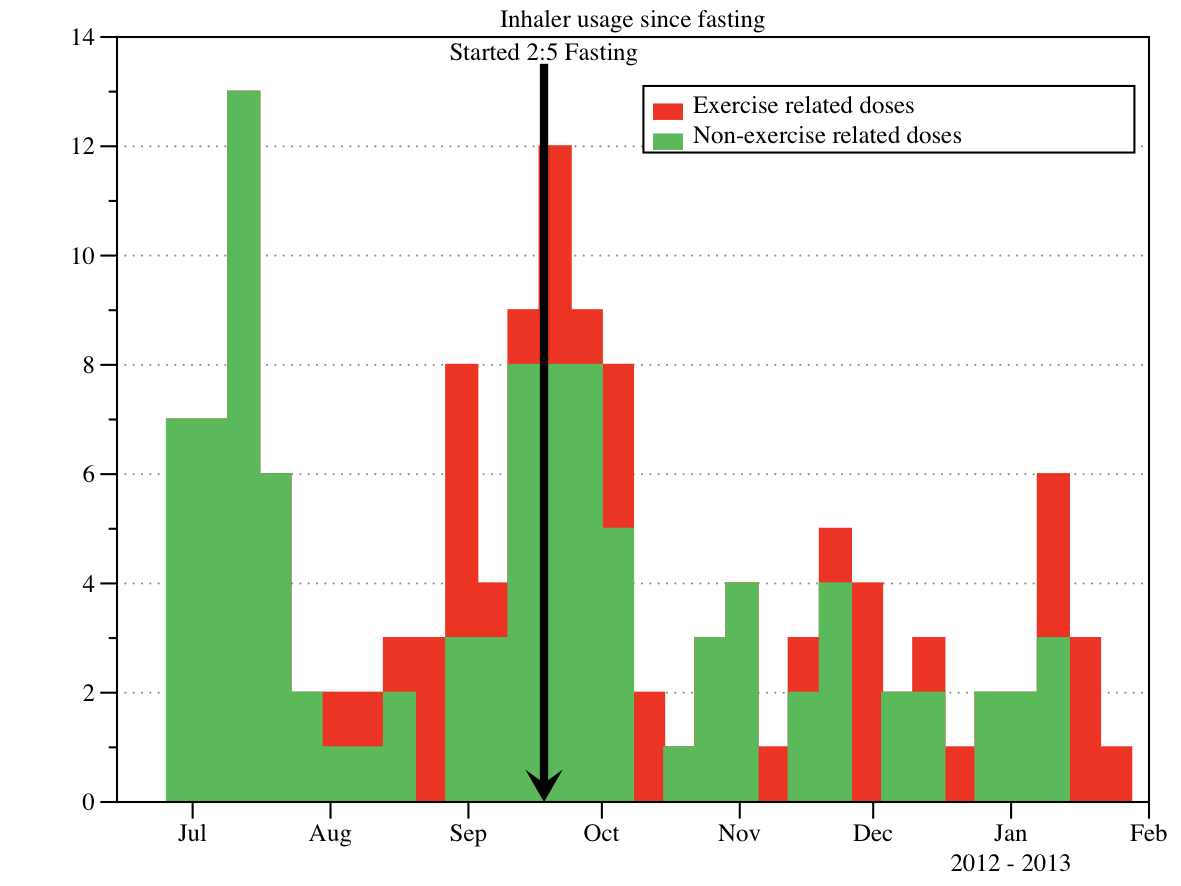
\includegraphics[width=\textwidth]{lifelog-inhaler-analysis}
\end{slide}


\begin{slide}
    \textcolor{blue}{\Large{Sleep vs Fasting}}

    \begin{itemize}
        \item Most in-depth analysis
        \item Code to loop through calendar and form table of data
        \item Use modelling program Wizard to inspect
    \end{itemize}

\end{slide}

\begin{slide}
    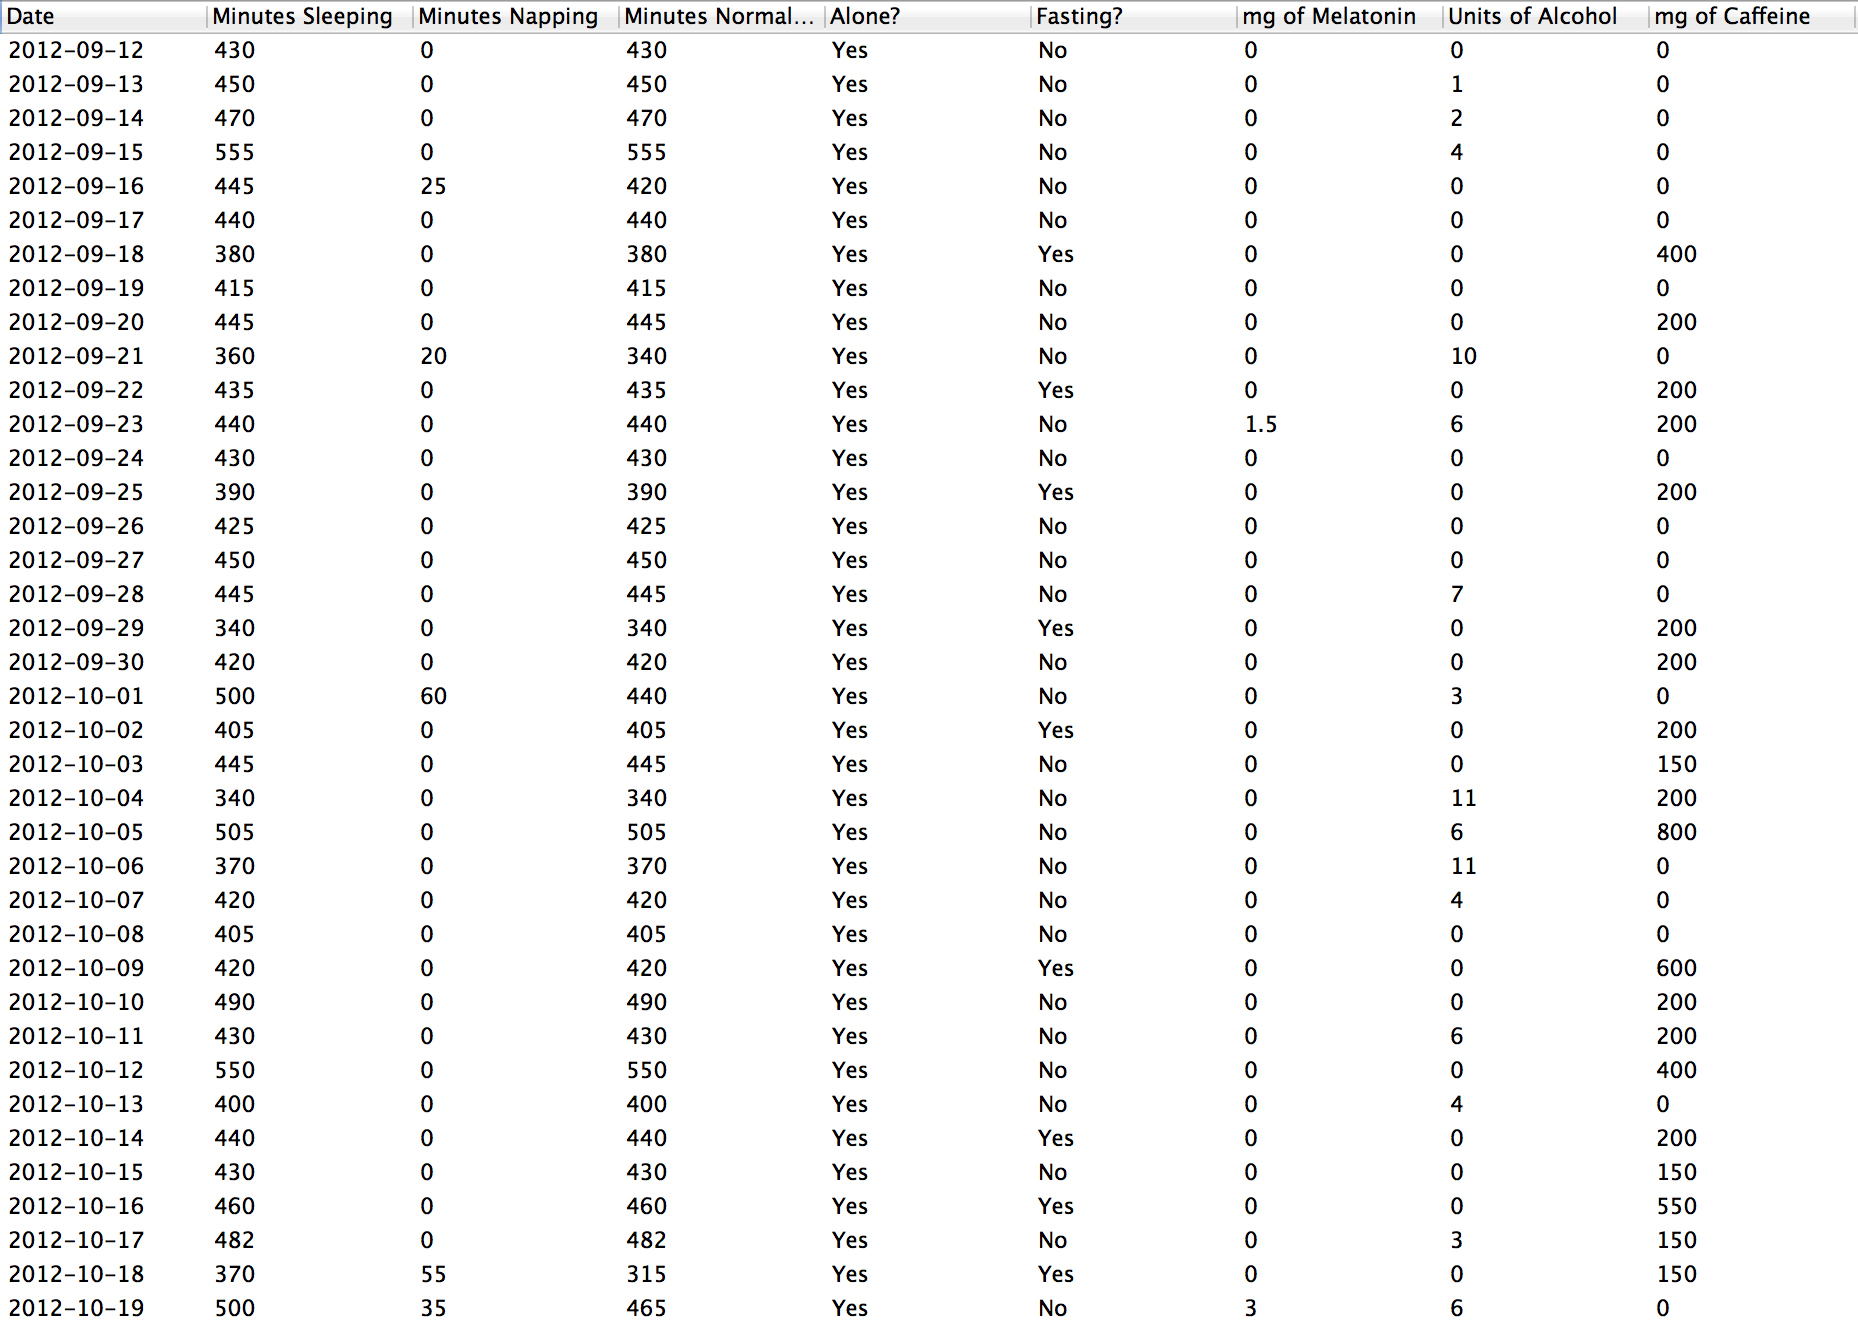
\includegraphics[width=\textwidth]{sleep-analysis-table}
\end{slide}

\begin{slide}
    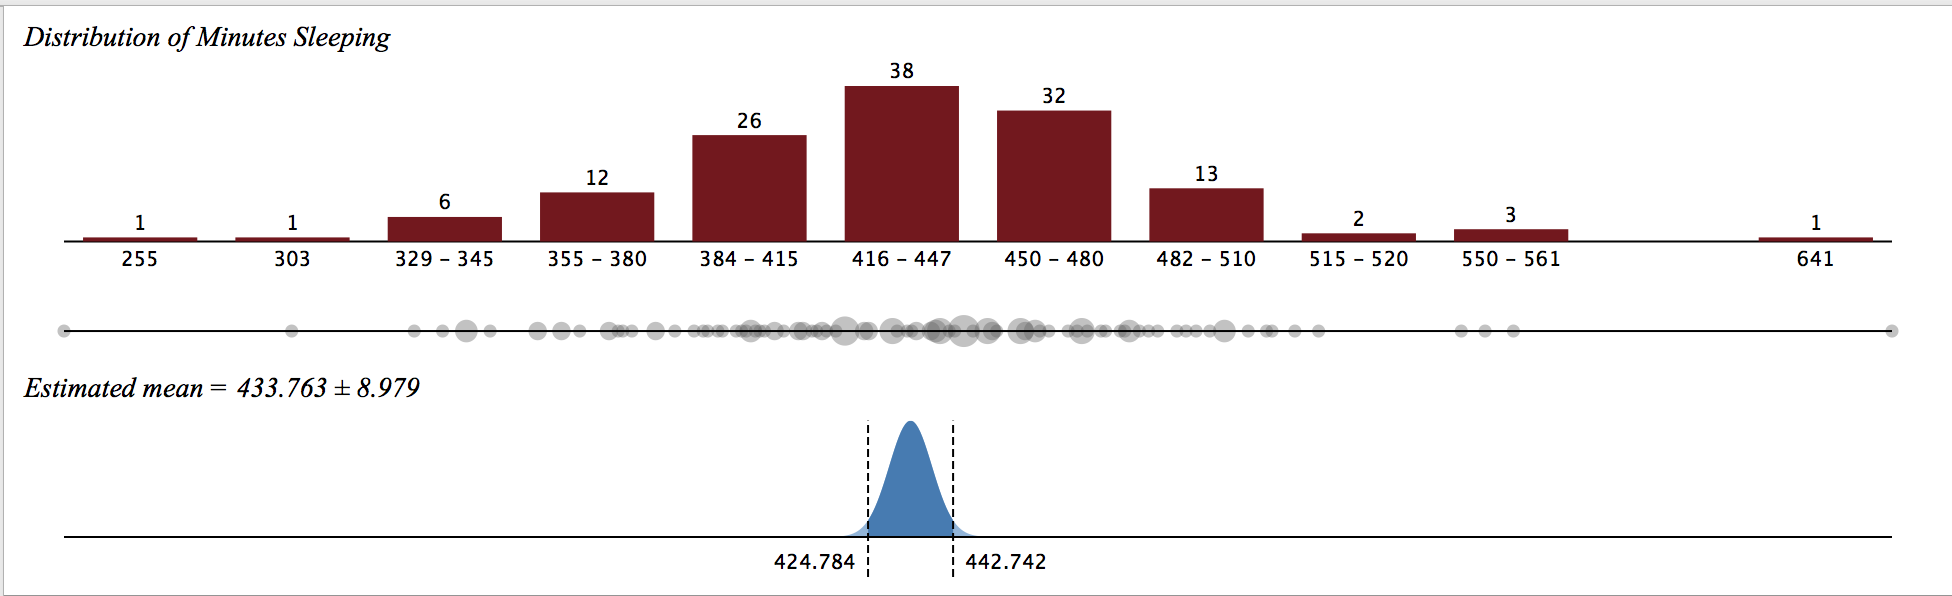
\includegraphics[width=\textwidth]{sleep-analysis-distribution}
\end{slide}


\begin{slide}
    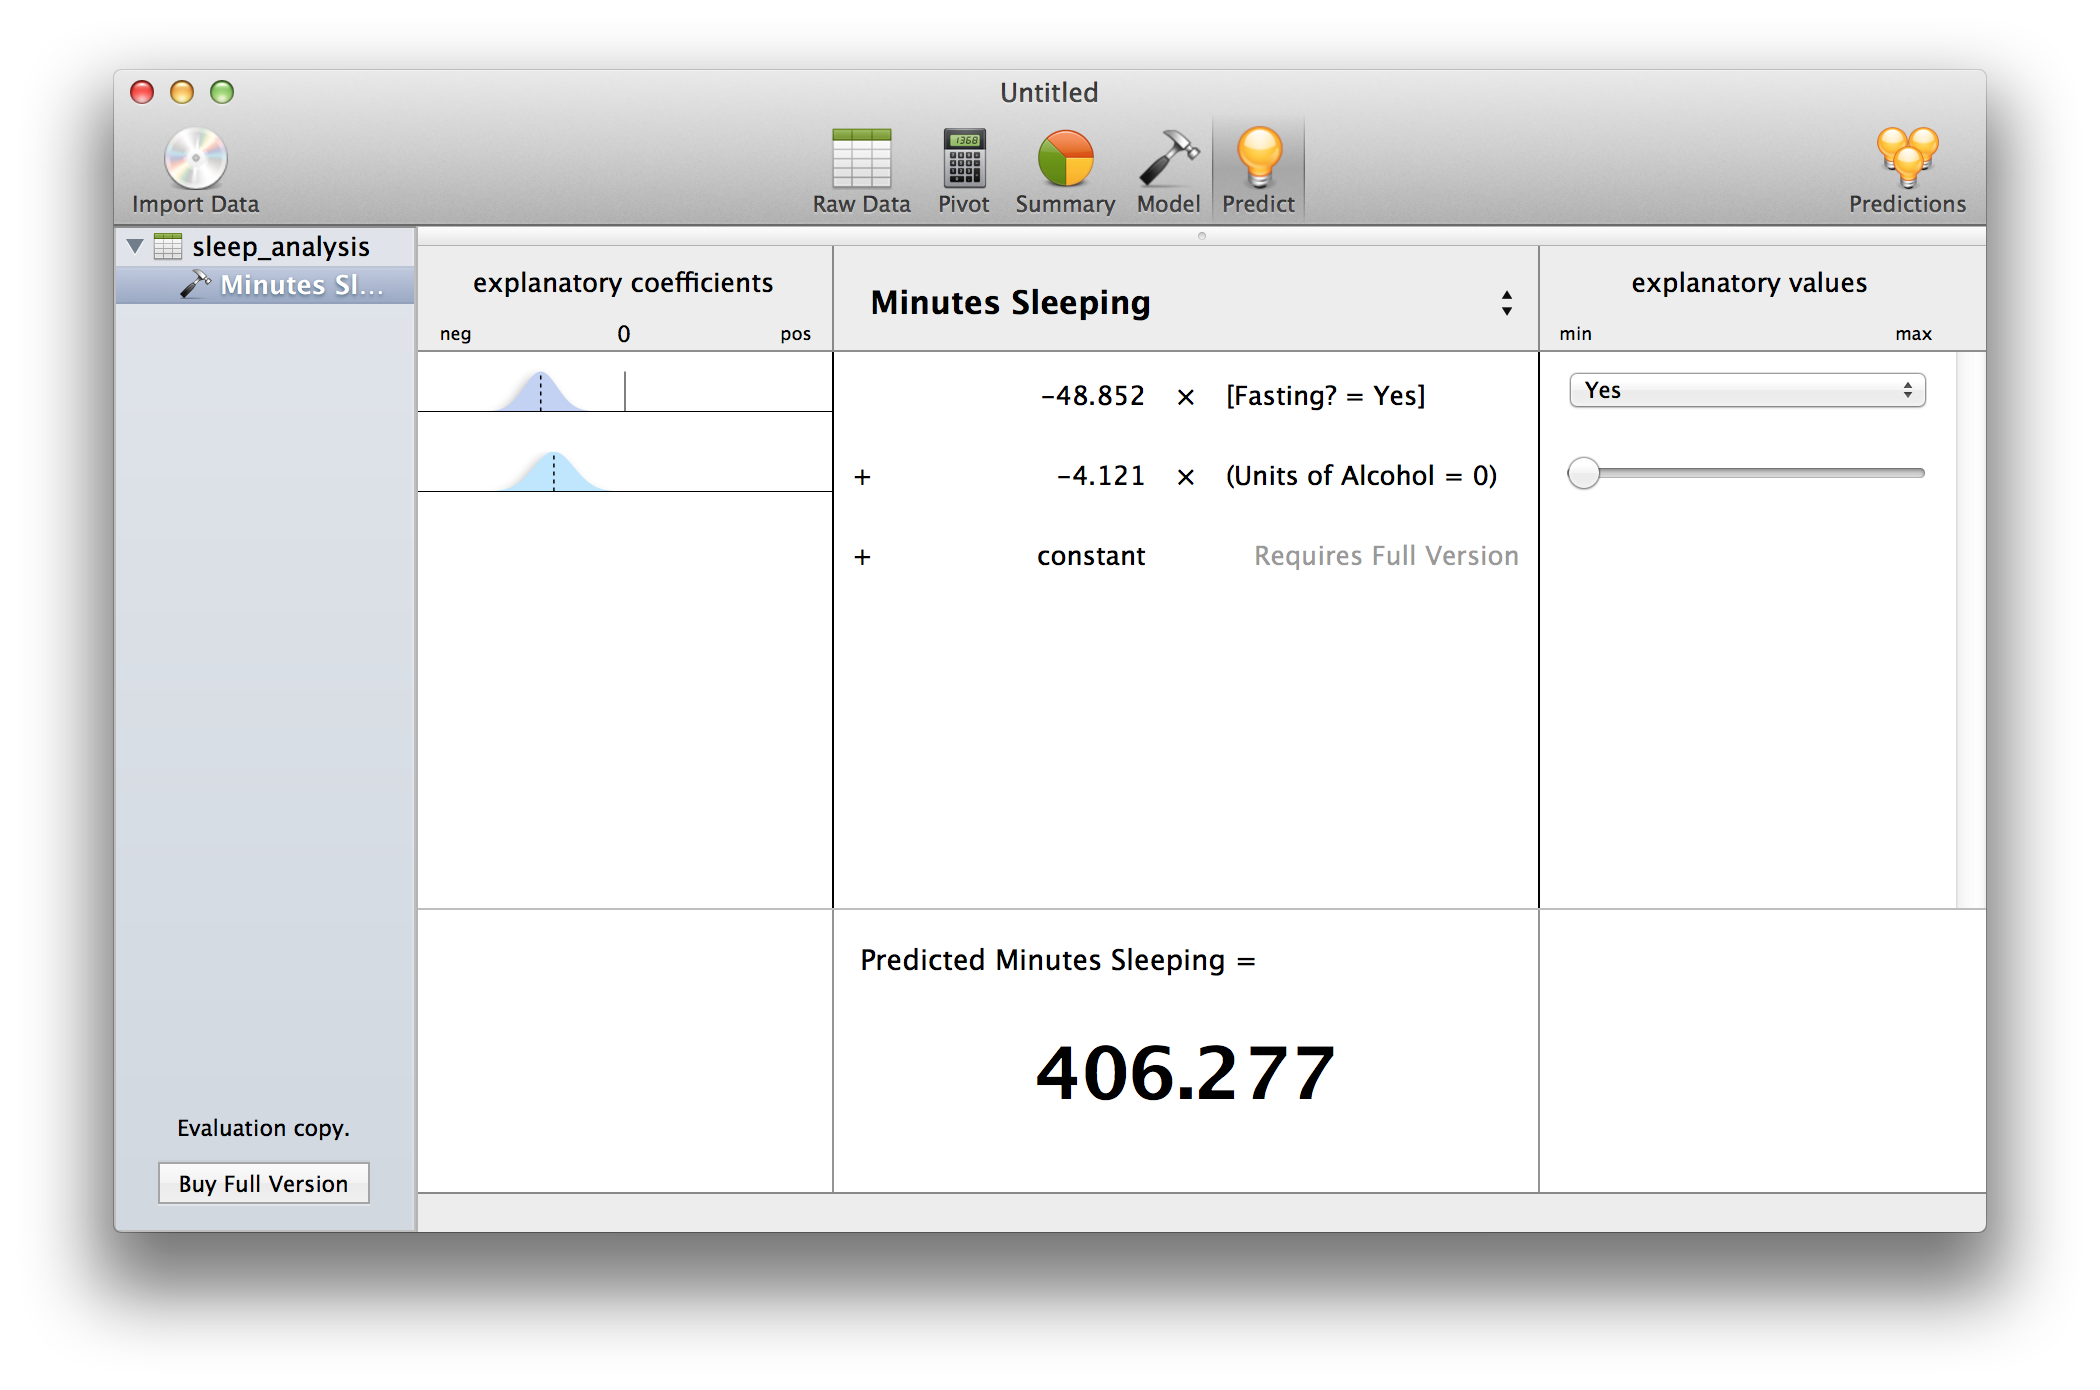
\includegraphics[width=\textwidth]{sleep-analysis-model}
\end{slide}

\begin{slide}
    \textcolor{blue}{\Large{Thank you}}

    \begin{itemize}
        \item \url{me@adamj.eu}
    \end{itemize}

\end{slide}



\end{document}
